\chapter{Introduction and Background Information}
\section{Motivation}
\label{sec:Motivation}
The motivation of this thesis is to show the methodology that can be used both by applied researchers and clinicians to draw meaningful survival and causal inference from imputed data. While all three fields (imputation, survival, causal)  are well studied, their interaction is not. I want the methods to be easy enough to describe to someone with a limited statistical background, but meaningful and valid so that the results obtained can be used in publication. The desire to have it this way stems from working on a related project with both statisticians and clinicians. While this thesis is motivated by cancer data, I believe that the methods used in this thesis are general enough to be applied to other types of data and situations.

\label{ch:Intro}
Missing data is a major problem in both statistics and medicine; however, it has not received attention proportional to its need. Survival analysis is well studied, but is relatively complete, so little new research comes out of this field. Propensity score analysis will help us determine causal relationships when we don't have a randomized controlled experiment. As one could imagine, all three of these fields are important to the applied statistician, as they will come across at least one at some point in their career.  The goal of this thesis is to demonstrate how to use all three in trio, a topic that has only received little interest in the literature. I will explain each of these three disciplines in detail before we dive into combining them.

\section{Imputation}
\label{sec:Imputation}
In an ideal world, we would have complete data with no missingness, however this is rarely ever the case. Imputation (specifically multiple imputation) is a way to ``fill in missing data'' with plausible values, and it forms the base of this thesis. All of the other analyses that will be used will follow from it, thus we need a solid understanding of it before we may proceed. Imputation itself has been around since the 1930's \cite{VanBuuren2012}, but multiple imputation is a recent development, proposed in the 1970's and formalized in 1987 by Donald Rubin \cite{Rubin1987}. To understand the use and importance of multiple imputation, we need to understand the problem of missing data, and the previous attempts to deal with it.

At first, statisticians paid no attention to missing data, and happily discarded records from their data that were incomplete. This procedure is known as complete case (CC) analysis. There are many problems with this paradigm. To begin with, you will lose a lot of statistical power when, because you are throwing away records and thus decreasing your sample size. In addition, this can be costly to the researcher. If it costs a set amount to collect a single record, and you don't use this record, you are wasting money. As well, in some rare cases, incomplete data might be the only type we can get (e.g. if we have a machine that analyzes a blood sample chemical level, but can't detect it if the level is too high or low). Lastly, and most importantly, we will be biasing our estimates if we discard them. For example, suppose we have a random sample of people and are testing a drug�s efficacy, and want to run a regression on some collected covariates. If men are known to not want to give all of their information, in the analysis, we will need to discard the male samples because they are incomplete, leaving us only with women. Thus, we no longer have a random sample, and will get biased results because we have knowingly thrown away half of our data which we know to be different \cite{VanBuuren2012}.

A slight improvement on this is called available case (AC) analysis. In this setting, a record is used in the analysis if it has all of the needed information for that analysis. So, a record could have missingness, but if the covariate with missingness is never used in the analysis, it will not be discarded. This paradigm is the standard analysis type for most statistical packages. It is better than complete case analysis, but is still flawed. We are still throwing away valuable data as we were with complete case analysis, although likely not as much. Available case analysis will still lead to bias in the same way that complete case did too. As well, new complications arise in available case analysis, namely that nonsensical situations like correlations outside of $\pm 1$, and inconsistent sample sizes for different analyses can arise.

The next wave of statisticians in the early $20^{th}$ century wanted to improve upon available case analysis, so they developed what we now call today imputation. Their specific incarnation was called single imputation, and their goal was to fill in missing values with a single plausible replacement value. A single method (such as regression, taking the mean, resampling) is used one time to impute or fill in the missing value. While this is a little better than complete case analysis, it still has many drawbacks. Asserting that a single value is the true value is unjustified. There is always some amount of error and uncertainty involved, and we can in no way be 100\% confident that our imputed value is correct. Furthermore, if I impute one value and you impute another, we may get completely different results from analysis on the data. This is obviously not a desirable trait.  In addition, imputing one time and calling it your true data will artificially increase your sample size. You are in effect treating the imputed values as if they were real, inflating your sample size with data that was not actually observed. This will give you unjustified statistical power and accuracy. While single imputation certainly has its drawbacks, the idea of actually trying to fill in the data is an important one, and multiple imputation fills in the gaps that single imputation is not able to cover.

Multiple imputation (MI) began in the 1970's, but it wasn't until 1987 when Donald Rubin formalized multiple imputation methodology in his seminal book \emph{ Multiple Imputation for Nonresponse in Surveys} did it start to gain acceptance \cite{Rubin1987}. The central idea is to frame the problem in a Bayesian framework, and produce $m\geq 2$ values to substitute in for each missing value, drawing these values from the missing covariates posterior distribution. Using these substitute values ($m$ values), we can think of the data now as being m datasets, each dataset containing the observed data, and one value for each piece of missing data. 

An example will make the MI process clear. Suppose that we had a dataset of age, weight, and height. We want to regress age on weight but we have missingness. First, we will impute our data (figure \ref{fig:miexample}, the first two columns). Once we have a sufficient number of datasets (we will talk about how to pick the number later), we can run out analyses on each of the MI datasets, treating the dataset as if it was complete (horizontal lines and third column). After running the model on the $m$ datasets, we can pool the results to get one single estimate with its associated variance (last column).  
\begin{figure}[!ht]
  \centering
    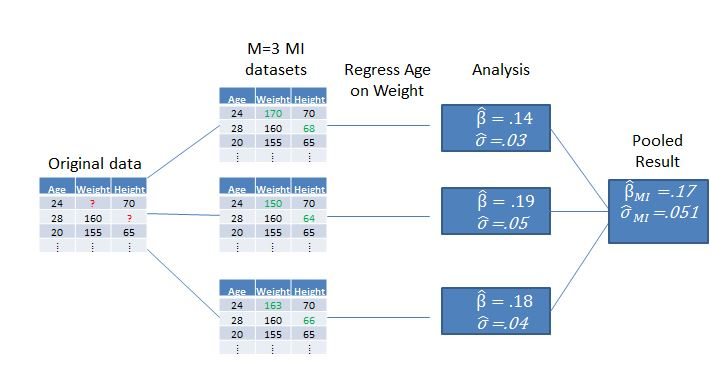
\includegraphics[width=0.8\textwidth]{mi_example_full.jpg}
  \caption{Visualization of MI data}
\label{fig:miexample}
\medskip
\small
In the original data, missingness is displayed by \textcolor{red}{?'s} and the imputed data is shown in the multiply imputed data as \textcolor{green}{\#'s}. We then regress age on weight, get the results from the individual datasets, and then pool them together.
\end{figure}


This method is obviously much better than the first two methods because it allows us to not throw away data, as well as to quantify our uncertainty about imputing the missing values. The only real drawback of multiple imputation is that we still don't have true data, but we can be confident enough in our estimations to compensate for that. The only better option would be to not have any missing data.

The use of multiple imputation has been steadily increasing over the past 30 years, and it is now the standard for missing data. Stef van Burren, an influential author in multiple imputation did a study of academic papers, and concluded that the number of publications using or mentioning multiple imputation is growing at an exponential rate since about 1990 \cite{VanBuuren2012}. Thus, using multiple imputation will be advised because of its popularity and strength.



\section{Survival}
\label{sec:Survival}
Survival analysis is a huge field, and there have been many textbooks written about it. I only plan to introduce the topics that are relevant to my case study.  For a much more detailed account of survival analysis, please see \cite{Klein1984}.

Survival analysis on the whole can generally be described as the analysis of time to event data, often in the presence of censoring or truncation (when we don't have complete information about the time of event).  There are many techniques used in this field, but the main tools that we will be using are Kaplan-Meier estimates, log rank tests, and Cox regression. 

Before we go on, it should be noted that often in the literature and software (and in this paper) we see terms like ``death/failure'' and ``survivors''. This is due to survival analysis being heavily influenced and intertwined with medical studies. A more general term for these would be ``event'' and ``those who have not had an event yet''. These terms are used because they are clear and concise, although it might not accurately describe the event at hand. For example, if we were tracking the time until a child loses all of their baby teeth; the term death would obviously not portray the event of interest, but may be used in the context to denote losing all of the teeth.

The Kaplan-Meier (KM) estimator is a nonparametric estimate of the true survival function (the probability that you survive after time t, $S(t)=P(T>t)=\int_t^\infty f(u)du$, where $f(u)$ is the unknown probability density function).  It is defined as 
$$\hat{S}(t)=\prod_{t_i<t}\frac{n_i-d_i}{n_i}$$
Where $n_i$ is the risk set, defined as the number of people who have not had the event or been censored right before time $t_i$ ,and $d_i$ is the number of deaths or events that you observe at time $t_i$ \cite{Kaplan1958}. The Kaplan-Meier estimator is very commonly used as a measure to see how different treatments affect the survival of the population in question, and is helpful in seeing at what time points survival changes the most (i.e. early or late). 

The log rank test is a popular nonparametric test that researchers often use to see if two or more survival curves come from the same distribution \cite{Bland2004}. This is a useful tool to have, because visualizing curves alone does not give us this information. We could have two curves that look radically different due to sampling error, yet still come from the same distribution. Knowing if the survival curves come from the same or different distribution is useful because it allows us to make statements like ``drug A is associated with longer survival time than drug B''.

The general log rank test is defined as:
$$\frac{\sum_{j=1}^{J}w_j(O_{1j}-E_{1j})}{\sqrt{\sum_{j=1}^{j}w_j^2V_{j}}}\sim N(0,1)$$
Where $w_j$ is the weight of each individual (must be $\geq 0$, we will set all to be 1), and $N_j=N_{1j}+N_{2j}$ is the number of subjects in the risk set at time j, composed from the sum of the number of deaths at time j in each group, $O_j=O_{1j}+O_{2j}$ is the observed number of deaths at time j, composed of the sum of deaths from either group at time j,  which leads to the desired quantities $E_{1j}=\frac{O_jN_{1j}}{N_j}$ , and $V_j=\frac{O_j(N_{1j}/N_j)(1-N_{1j}/N_j)(N_j � 0_j)}{N_j -1}$

Since we set all of the weights to be 1, this test, as it is, places equal weight to all of the deaths we observe. We could change these weights though to give more emphasis to certain death times. This is useful for example if we have a drug that takes a long time to start working. We wouldn't care about early deaths, only about later times when we are comparing the survival. Putting more weight on the later deaths would help to answer this question better. It can be proven that the log rank test is equivalent to the score test on a Cox model (which will be discussed next) fit the same data with no ties \cite{Klein1984}.

Proportional hazards regression, often called Cox regression or Cox model is a modelling tool that allows us to analyze the hazard ratio of a covariate, assuming that each covariate acts to multiply the hazard ratio. 

The hazard function is a survival tool that tells us the rate of events at time $t$, conditional on survivorship until time $t$. Mathematically, it is given by:
$$\lambda(t)=\lim_{\Delta t\rightarrow 0+}\frac{P[t\leq T<t+\Delta t|t \leq T]}{\Delta t}$$.
Cox regression is a maximum (partial) likelihood method estimator, given by: 
$$h(t|Z)=h_{0}(t)\exp(\sum_{k=1}^{p}\beta_{k}Z_{k})$$.
where $h_0(t)$ is what's known as the baseline hazard, and can be any positive function , and often times a parametric model like the Weibull is chosen. Note how it only depends on time and not any covariates.  Z is a vector of observed covariates, and does not depend on time. The $\beta$�s are found by maximizing the partial likelihood function
$$L(\beta)=\prod_{i=1}^{D}\frac{\exp(\sum_{k=1}^{p}\beta_{k}Z_{(i)k})}{\sum_{j\in R(t_{i})}\exp(\sum_{k=1}^{p}\beta_{k}Z_{jk})}$$
Where $Z_{(i)k}$ is subject i's kth covariate, $R(t_j)$ is the risk set (set of those who have not died yet at the time just prior to $t_j$), D is the number of distinct death times and p is the total number of covariates in the model. The betas are maximized by the Newton-Raphson method \cite{Cox1972}.

Our inference of interest is the hazard ratio, given by 
$\frac{h(t|Z)}{h(t|Z^{*})}=\exp(\sum_{k=1}^{p}\beta_{k}(Z_{k}-Z_{k}^{*}))$
Where Z* is another set of covariates. The relative risk (or hazard ratio) describes how the hazard changes between individuals with different covariates. Often times, the interest lies in what happens when all covariates are held constant, and the covariate of interest is increased one unit. This ratio will be a constant, and should not vary over time; hence the name proportional hazards. This is so because the ratio does not depend on the baseline hazard (which cancels out when taking the ratio). Using Cox regression, statements such as   ``Increasing the drug by one \textit{mg} will decrease the rate of death (compared to non-users) by 30\%''. Cox modelling is one of the most used models in survival and medical literature.

\section{Causal Analysis}
\label{sec:PSA}
Readers: please note that this is the weakest section. I plan to make it more thorough as my research progresses.


Although we can analyze any observational data using survival analysis, unless a randomized controlled trial is conducted, we cannot make any claims about causality. In order to prove causality, we need experimental data, not observational data. In an ideal world we would like to be able to do research and say that A causes B, rather than ``our study says that A is associated to B''.  However, the only way to get this interpretation is if we conduct a randomized controlled trial.

Randomized controlled trial (RCT) is a term that is often thrown around, but I want to be precise with its definition. In the simplest example, RCT is an experiment where subjects (with no knowledge of the experiment) are randomly assigned to either the treatment of the control. Thus, the only difference between the subjects should be the fact that they have or have not received the drug. This is in stark contrast to a retrospective study of observational data, where historic data of people who chose what group/ treatment they wanted to be in are studied. When making judgment on a retrospective study, we cannot be sure if the differences between the groups are due to their treatment choice, or some other factor. RCT's are the gold standard for experiments, and should be used if possible. But often times monetary, ethical, or other factors prevent us from doing so. In this case, the best data we may be able to get is retrospective study. 

However,  we can frame our problem in a framework known as the Rubin Causal model, which helps get causal understanding from non-experimental settings \cite{Guo2010}. In this model, the goal is to balance the groups as much as possible, so the only difference is due to the treatment in question. In an ideal world, we would like to observe both potential outcomes (i.e. how the subject would respond to the treatment and to the control, denoted $Y_i(0),Y_i(1)$ for subject i). This is obviously not possible, since we can only observe one outcome. But we can get a good idea of the treatment effect by taking the difference of the average treatment effect between the two groups, known as the average treatment effect (ATE).  
%I plan to elaborate on this much more in the future.


There are many ways to implement Rubin's causal model, but the most popular is known as \textit{propensity score analysis}. The propensity score is the probability that the subject received the treatment given the subjects covariates. It is computed using the patient's baseline (pretreatment) information \cite{Rosenbaum1983}.  We assume that some of the covariates play a role in deciding how the patient chooses the group, so controlling for this makes all of the patients seem similar. Propensity scores lead to group balancing, that is, if propensity scores are controlled, then our groups will have the same distribution at the baseline. And thus, we can treat the data like it was an RCT. The two most popular propensity score methods are propensity score matching (where we match those who picked the treatment to those who did not based off of propensity score) and propensity score weighting (where each individual's contribution to the average treatment effect is dependent on the inverse of their propensity score). Propensity score matching has fallen out of favor recently because there will be some data thrown away, and the balancing that takes place might not be that accurate \cite{King2015}. However, propensity score weighting is still a popular method.

Getting the propensity score is often done by logistic regression, although newer methods include regression trees and other binary classifiers. The propensity score for the $i^{th}$ individual is given by:

$$\hat{e}_i(z)=p(T_i=1|Z_i)$$
where $T_i$ is treatment (1 means the subject got treatment), and $Z_i$ are their covariates. There has been a lot of debate as to which covariates to include in the propensity score; either all variables, or only relevant variables. I don't aim to settle this debate in this paper. 

Propensity scores use is justified by the propensity score theorem, which states that if we assume conditional independence of the treatment given covariates on the outcomes, then we can also assume conditional independence of the treatment given the propensity score on the outcomes. Symbolically
$$(Y(0),Y(1))\perp T|X\implies(Y(0),Y(1))\perp T|p(X)$$
where the Y's denote the potential outcomes. If this is the case, then the potential outcomes are independent of the treatment given the covariates. We need this to hold, because it allows us to break the connection between the covariates and the treatment choice \cite{Angrist2008}.

Now we have the probability or propensity of a subject being assigned to a specific treatment given their covariates. Its usefulness is immediately seen in the matching case, because now instead of matching on $n$ different levels, we need only to match on one number, the propensity score. 

This paper is interested in weighting though, specifically, inverse probability of treatment weight (IPTW). These weights are given by
$$w_i=\frac{T_i}{\hat{e}_i(z)}+ \frac{1-T_i}{1-\hat{e}_i(z)}$$
where T is the treatment and Z is the covariate. This might be unstable as propensity scores approach 0 or 1, so alternate methods such as stabilized weights by Cole and Herman or trimmed weights have been presented that reduce this issue \cite{Austin2014}. 
%!! elaborate on this later!!

Once the IPTW is calculated, we need to check how much balancing was actually achieved. We can do so by observing the change in standardized bias, standardized difference, or graphically on a histogram of propensity scores \cite{Harder2011}. Once the weights are calculated, we can add them to our model and get out causal results and inferences such as the ATE.
\begin{comment}
We are not out of luck though, because by using Rubin's causal model, we can talk about causation in this setting. Our goal is to determine the causal effect of a treatment.  To do so, we need to have a completely randomized experiment, where the differences in the groups outcome can only be attributed to the differences in the treatment. When we have a non randomized experiment, we incur bias, because differences can come from things besides the treatment. Under Rubin's causal model, we aim to balance the groups out so that it is like there was random assignment. Our ultimate goal is to look at each subject and see how they react to the treatment and to the control. This is obviously impossible, since a person cannot at the same time take the treatment and control. This is what's called the fundamental problem of causal inference. We can only observe one outcome and that is the issue. We need what is known as the counterfactual, or the other potential outcome. We go about getting this by matching a subject with a set of covariates to someone who is very similar from the other group. We then look at all of the subjects differences to see if there truly is a causal effect.
\end{comment}
